\begin{frame}
\frametitle{Outline} 
\tableofcontents
\end{frame}

\begin{frame}
\transdissolve<2->
\frametitle{Set-theoretic types}

We consider the following possibly recursive types:

{\Bl$$\T\ ::=\  \Bool\,\mid\,\Int\,\mid\,\pair\T\T\,\mid\,\T\To\T \,\mid\,{\color{darkgreen}\T\Or\T}\,\mid\,{\color{darkgreen}\T\!\And\!\T} \,\mid\, {\color{darkgreen} \neg\T}\,\mid\,{\color{darkred}\Any}\,\mid\,{\color{darkred}\Empty}\,\color<1>{white}\mid\,~\textcolor<2>{magenta}{\alpha} \color<2>{white}\,\mid\, \color<3>{magenta}{c} $$}

\pause\pause\pause\pause\pause
\bigskip

\textbf{Necessary to precisely capture the programming style used with dynamic languages:}
\begin{enumerate}
\item non-uniform structures/branching (union types, singletons)
\item overloading (intersection types)
\item pattern matching (negation types, ...)
\end{enumerate}


\textbf{\color<-6>{white}\color<7>{darkslateblue}Let us see each point more in detail}

\bigskip

\vfill

\small\color{gray} Note: henceforward I will sometimes use $\Bl\T_1\texttt{|}\T_2$ to denote $\Bl\T_1\Or\T_2$

\only<2>{\begin{textblock}{5}(0,0)
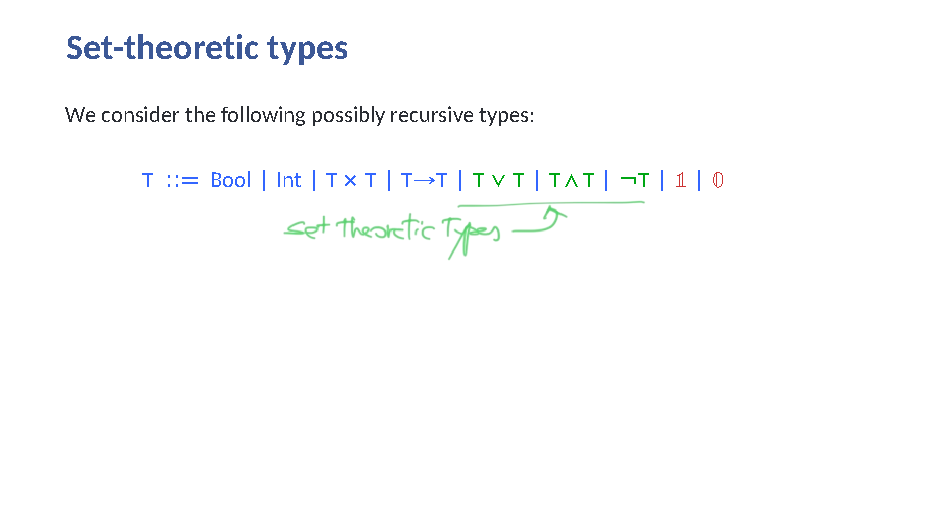
\includegraphics[scale=1]{images/slide-settheore.pdf}
\end{textblock}}
\only<3>{\begin{textblock}{5}(0,0)
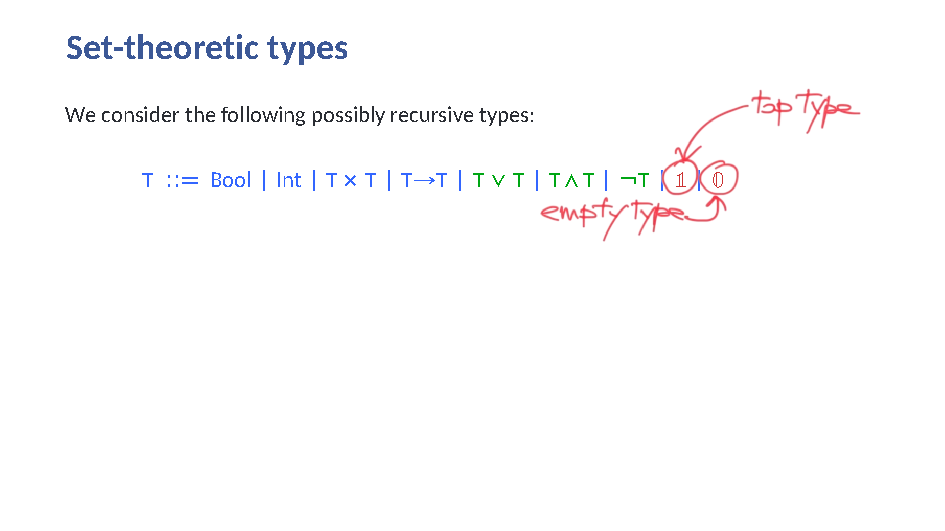
\includegraphics[scale=1]{images/slide-topbottom.pdf}
\end{textblock}}
\only<4>{\begin{textblock}{5}(0,0)
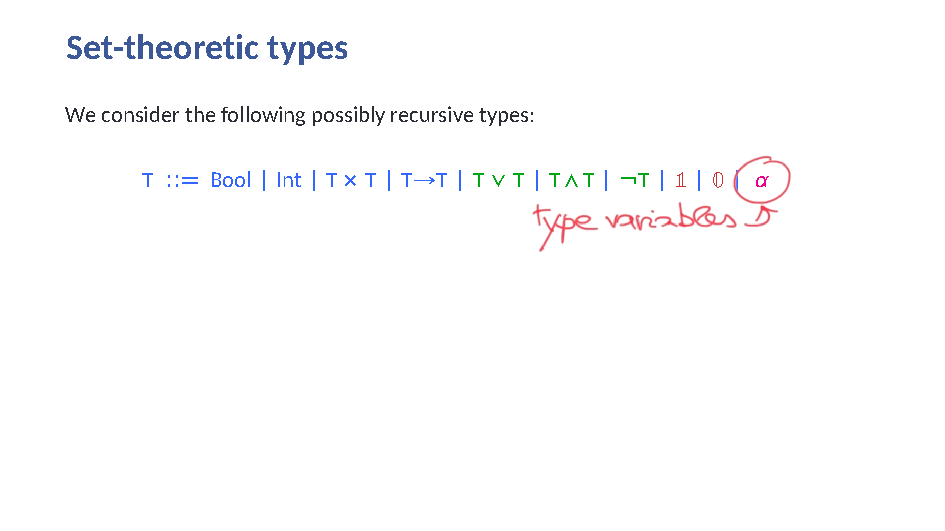
\includegraphics[scale=1]{images/slide-variables.pdf}
\end{textblock}}
\only<5>{\begin{textblock}{5}(0,0)
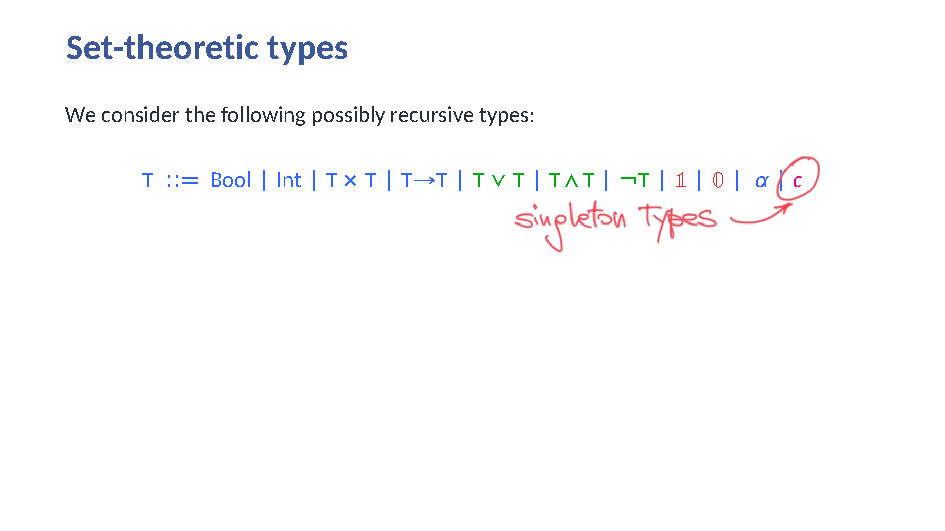
\includegraphics[scale=1]{images/slide-singleton.pdf}
\end{textblock}}
\end{frame}

\subsection{Branching, overloading, and pattern matching}

\begin{frame}[fragile]\transdissolve
\frametitle{1. Branching and discriminated unions}\vspace{-4mm}
\small
\begin{minted}{TypeScript}
type Status = "pending" | "success" | "error";
type Result = string | number | boolean;
function processStatus(input: Status): Result {
  switch (input) {
    case "pending":
      return "Processing...";       // returns string
    case "success":
      return 200;                   // returns number
    case "error":
      return false;                 // returns boolean
    default:
      return "Unknown status";      // returns string
  }
}
\end{minted}
\pause


% Discriminated unions are a common pattern in dynamic languages to handle different types of data structures that share some common properties.
\begin{minted}{TypeScript}
type PaymentMethod = 
  | { type: "credit_card"; cardNumber: string; cvv: string }
  | { type: "paypal"; email: string }
  | { type: "bank_transfer"; accountNumber: string; routingNumber: string };
\end{minted}
\end{frame}



\begin{frame}[fragile]\transdissolve
  \frametitle{2. Overloading: basic use}
 \structure{\bf Aka \emph{ad hoc} polymorphism: functions that execute different code on arguments of different types}

\smallskip

\begin{minted}{TypeScript}
function double (x) {
    return (typeof(x) === "number") ? 2*x : x.concat(x);
}
\end{minted}
\textcolor<4>{red}{If applied to an integer returns an integer, if applied to a string returns a string}
  \pause
\begin{exampleblock}{Use set-theoretic types}
  \begin{itemize}
    \pause
     \item Naive solution: union types
       \centerline{\pb{(number|string)$\to$(number|string)}}
       \pause\pause
     \item Better solution: intersection types
       \centerline{\pb{\color<6>{darkred}(number$\to$number) \& (string$\to$string)}}
  \end{itemize}
\end{exampleblock}
\end{frame}


\begin{frame}[fragile]
\frametitle{2. Overloading: advanced use}
\begin{minted}{TypeScript}
function toBoolean(x) {
    if (x === 0 || x === "" || x == null || Number.isNaN(x)) return false;
    return true;
}

function logicalOr(x, y) {
    if (toBoolean(x)) return x; return y;
}
\end{minted}
\pause

\bigskip

\begin{exampleblock}{Fine grained typing to capture the code semantics}
\color{typeBlue}
\tt
type Falsy = 0 | "" | null | undefined | NaN;

type Truthy = $\neg$Falsy;

toBoolean : (Truthy $\to$ true)  $\wedge$ (Falsy $\to$ false)

logicalOR : \ (($\alpha{\wedge}$Truthy$\,\times\,\Any$)$ \to \alpha$)  $\wedge$ ((Falsy$\times \beta$)$\,\to \beta$)

\end{exampleblock}
\end{frame}




\begin{frame}[fragile]
\frametitle{3. Precise typing of pattern matching (I)}
Consider the following pattern matching expression
 
\hspace*{5mm}{\Bl$\texttt{ match }  e  \texttt{ with } p_1 \texttt{ -> } e_1 \texttt{ | } p_2\texttt{ -> } e_2$}

where patterns are defined as follows:
\centerline{$\Bl p ::= x \ \mid\  \patpair{p}{p} \ \mid\ \pator{p}{p}\ \mid\ \patand{p}{p} $}
\pause
If we interpret types as set of values
\centerline{$\Bl
t = \{ v\mid v\text{ is a value of type }t\}$}
\pause
then \textbf{\color{darkslateblue}the set of all values that match a pattern is a type}
\centerline{\color{magenta}
$\accept{p} = \{ v\mid v\text{ is a value that matches }p\}
$}
\vspace{-9mm}
{\color{lightgray}
\begin{eqnarray*}
\accept x  & = & \Any\\[-1.5mm]
\accept{\patpair{p_1}{p_2}}  & = & \pair{\accept{p_1}}{\accept{p_2}}\\[-1.5mm]
\accept{\pator{p_1}{p_2}} & = & {\accept{p_1}}\Or{\accept{p_2}}\\[-1.5mm]
\accept{\patand{p_1}{p_2}} & = &{\accept{p_1}}\And{\accept{p_2}}
\end{eqnarray*}
}
\pause\pause\vspace{-9mm}

\textbf{\color{darkslateblue}Let us see how to type pattern matching.}
\only<4>{\begin{textblock}{5}(0,0)
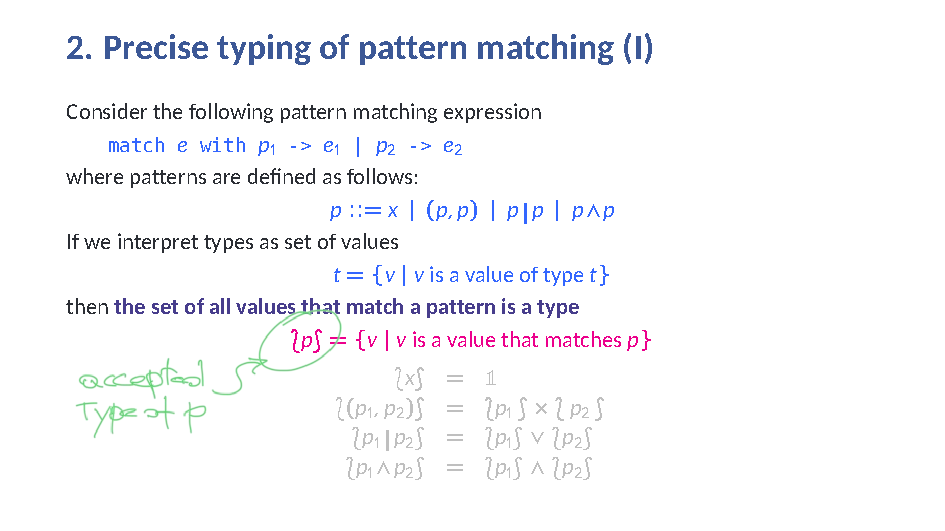
\includegraphics[scale=1]{images/slide-accepted.pdf}
\end{textblock}}
\end{frame}



\begin{frame}
\frametitle{3. Precise typing of pattern matching (II)}\transdissolve<10>

\textbf{Boolean type connectives are needed to type pattern matching:}

\pause
\smallskip

    \hspace*{5mm}{\Bl$\texttt{ match }  e  \texttt{ with } p_1 \texttt{ -> } e_1 \texttt{ | } p_2\texttt{ -> } e_2$}\pause

   \smallskip

Suppose that $\Bl e:\T$ and let us write $\Bl\T_1\setminus\T_2$ for $\Bl\T_1\!{\And}\!\neg{\T_2}$\\[-2mm]

\pause

  - To infer the type $\Bl\T_1$ of $\Bl e_1$ we need {\color{blue}$\T{\color<8->{magenta}\mypmb<8->{\And}}\accept{p_1}$};

\pause

  - To infer the type $\Bl\T_2$ of $\Bl e_2$ we need {\color{blue}$(\T{\color<8->{magenta}\,\mypmb<8->{\backslash}}\accept{p_1}){\color<8->{magenta}\mypmb<8->{\And}}\accept{p_2}$;}

\pause

  - The type of the match expression is {\color{blue}$\T_1{\color<8->{magenta}\mypmb<8->{\Or}} T_2$ }.

\pause

  - Pattern matching is exhaustive if $\color{blue}\T\leq\accept{p_1}{\color<8->{magenta}\mypmb<8->{\Or}}\accept{p_2}$;


\pause\pause
\textbf{Formally:}
\vspace{-2mm}
\begin{mathpar}\Bl
\infer[{[Match]}]
{\Gamma\vdash e:\T\and\Gamma, \T\!\!\And\!\!\accept{p_1\!}/p_1\vdash e_1:\T_1\and \Gamma, \T\setminus\accept{p_1\!}/p_2\vdash e_2:\T_2}
{\Gamma\vdash \texttt{match } e \texttt{ with }p_1 \texttt{->} e_1 \texttt{ | }p_1 \texttt{->} e_2 : \T_1\Or\T_2 }\mbox{\small($\T\leq\accept{p_1\!}\Or\accept{\!p_2\!}$)}
\end{mathpar}
\vspace{-4mm}

\small\color{gray}
where $\Bl \T/p$ is the type for the capture variables in $\Bl p$ when it is matched against values in $\Bl \T$.

\only<10>{\begin{textblock}{5}(0,0)
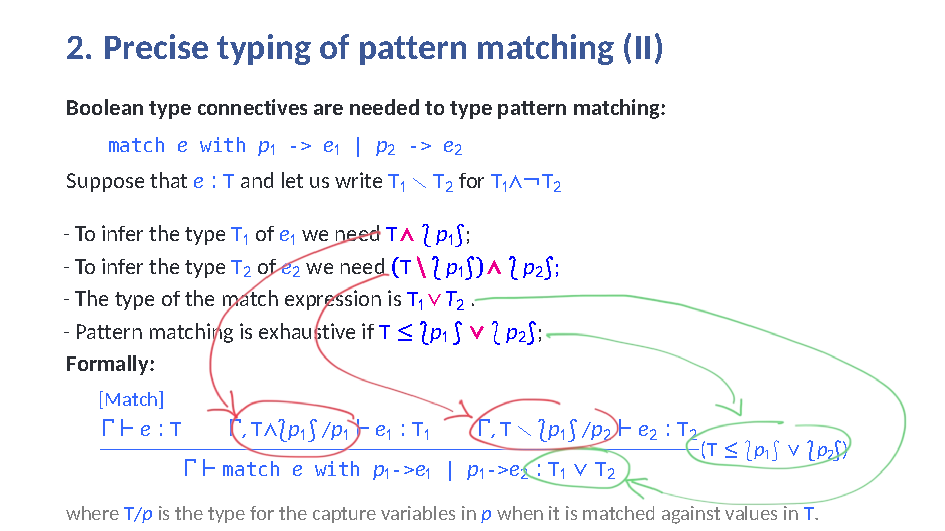
\includegraphics[scale=1]{images/slide-caseexp.pdf}
\end{textblock}}
\end{frame}

\subsection{Semantic subtyping}
\begin{frame}
\frametitle{Semantic subtyping}

Many dynamic languages support union and intersection types: TypeScript, Flow, Hack, Python, Julia, and Ceylon. Negation types are less common: TypeScript (with the `Exclude` utility type) and Scala (with `Not` type constraints).

\pause\bigskip

\textbf{What differentiates our approach is the use of \emph{semantic subtyping} to define\\  the subtyping relation for union, intersection, and negation types.}

\bigskip

\begin{enumerate}
  \item<3-> Define a set-theoretic interpretation of types as sets of values
  \item<4-> Define union, intersection, and negation types as set-theoretic operations
  \item<5-> Define the subtyping relation as a set-theoretic inclusion relation
  \item<6-> Deduce from this how to decide the subtyping relation and compute type operators
  \end{enumerate}

\end{frame}

\begin{frame}\transdissolve
\frametitle{Semantic subtyping: in practice}
\pause
\begin{enumerate}
\item<2-> $\begin{array}[t]{lcl}
  \sem{Int} & = & \{ n \mid n \text{ is an integer} \}\\[-1mm]
  \sem{Bool} & = & \{ \texttt{true}, \texttt{false} \}\\[-1mm]
  \sem{\T_1\to\T_2} & = & \{ f \mid v\in\sem{\T_1}\implies f(v)\in\sem{\T_2} \}\\[-2mm]
  &\vdots
\end{array}$
\item<3-> ~~$\sem{\T_1\Or\T_2} = \sem{\T_1}\cup\sem{\T_2}, \quad
\sem{\T_1\And\T_2} = \sem{\T_1}\cap\sem{\T_2}, \quad
\sem{\neg\T} = \{ v \mid v\notin\sem{\T} \}$\\[4mm]
\item<4-> ~~$\T_1\leq\T_2 ~~\stackrel{def}{\Longleftrightarrow}~~ \sem{\T_1}\subseteq\sem{\T_2} ~~\Longleftrightarrow ~~ \sem{\T_1}\cap\sem{\neg\T_2}=\varnothing ~~ \Longleftrightarrow ~~ \T_1\And\neg\T_2\leq\Empty$\\
\item<5-> $\color{cadmiumgreen}
\begin{array}{l}
\displaystyle
\syncap_{i \in I} t_i \syntimes s_i \leq
  \syncup_{i \in J} t_i \syntimes s_i ~~\iff~~
\forall J' \subset J.~
\left(
\syncap_{i \in I} t_i \leq \syncup_{i \in J'} t_i
\right)
\mbox{or}
\left(
\syncap_{i \in I} s_i \leq \syncup_{i \in J \backslash J'} s_i
\right)
\end{array}
$
\end{enumerate}
\pause\pause\pause\pause
\begin{block}{Paying the price}
  \begin{itemize}\color{newgreen}
    \item[\textcolor{newgreen}{\ding{52}}] Unions, intersections, and negations are \emph{\sl really} set-theoretic\color{red}
    \item[\textcolor{red}{\ding{56}}] Simply extending syntactic subtyping is not an option
  \end{itemize}
\end{block}

\end{frame}



\begin{frame}
\frametitle{Theoretical foundations}
\begin{itemize}
\item<1-> Semantic Subtyping for Set-Theoretic Types (JACM 2008)    
\item<2-> Polymorphic Types and Subtyping (ICFP 2011)
\item<3-> Typing of Polymorphic Functions and Local Type Inference (POPL 2014, POPL 2015)
\item<4-> Gradual Typing (POPL 2019)
\item<5-> Monomorphic Type Reconstruction (POPL 2022)
\item<6-> Uniform Typing for Records and Dictionaries (ICFP 2023)
\item<7-> Polymorphic Type Reconstruction and Occurrence Typing (POPL 2024)
\item<8-> Row Polymorphism (OOPSLA 2025)
\item<9-> First-class Modules (in progress)
\end{itemize}
\end{frame}

\begin{frame}
\frametitle{Set-theoretic types: state of the art}
\transdissolve<2>
\includegraphics<1>[width=.7\textwidth]{images/POPL24 1.png}
\includegraphics<2->[width=.7\textwidth]{images/POPL24.png}
\only<3>{
\begin{textblock}{12}(2.9,7.8)\small\color{purple}
    $\forall(\alpha{\leq}\texttt{Truthy})\forall(\beta)\,.\, (\alpha,\texttt{Any}\to\alpha)\wedge(\texttt{Falsy},\beta\to\beta)$
\end{textblock}
\begin{textblock}{12}(2.9,12.3)\small\color{purple}
    $\forall(\alpha)\forall(\beta)\forall(\gamma)\,.\, ((\alpha\to\beta)\to((\alpha\to\beta)\wedge\gamma))\to((\alpha\to\beta)\wedge\gamma)$
\end{textblock}}
\end{frame}
